\chapter{Why}

\section{Doubt and Faith}

\keywords{compulsive thoughts, orientation of views, unexpected changes}

The interest in meditation practice is often started by feelings of
suffering, we feel the need to deal with a disturbing or painful
experience. We know `something is wrong' and we can't shake it off, or
it could be the pain of loss creating a sense of confusion where nothing
makes sense -- such feelings keep returning, they don't let themselves
be ignored. Instead of answers, only the thinking keeps going round and
round: `Why does it have to be like this? What should I do, and why?
What's the point?'

We don't care much for alertness and right view until life makes us
realize how much confusion and pain is caused by a view which is not
aligned with the way things are. Even in such confusion, merely
acknowledging the state of inner chaos to ourselves already starts to
provide some order and orientation.

It is like when driving on a road cluttered with trash. Slowing down to
look around is already much better then being blind to the dangerous
clutter. Our head is full of thoughts but only few of them indicate
reliable directions, so we better examine them. Previously we held a
view that things in our world are one way, but they have changed in a
way we didn't expect. It is not their fault, it is not our fault, but
the unexpected change is confusing, and we have to adjust our view.

Experiencing impermanence pulls the carpet out from under our feet, but
at the same time transforms our values, the qualities which we seek out
as valuable in our experiences. If we don't understand the change, it
causes confusion, which is followed by doubt. Even though we might know
what we \emph{should be doing}, but we get stuck in the sense of doubt
and meaninglessness and we can't even begin.

\keywords{meaning, choosing beliefs}

Why do you get up in the morning to do anything? Why does it matter at
all? If I keep asking `why' and dig into the layers of my constructed
self like this, the first layer reveals a matter of habit, `because this
is what I did yesterday too'. Under that, the answers are formed out of
stories I tell myself about myself and the world I live in. Under that,
some reasoning, philosophy and abstract ideas. Under that, I am
desperately trying to hold onto something, and I struggle by defending
my ideas with personal memories and experiences (`because when I was
like this and this \ldots{}'), or referring to famous names (`because
teacher so-and-so said \ldots{}'). Under that, I have to give up and
confess that it is a matter of faith and personal conviction. It is
simply what I decided there and then. At the end I stand there and
\emph{I don't know}, but \emph{I believe} that doing so makes sense.

Faith is not a fixed quality in the mind, we have the capacity to choose
credible statements which we perceive to be guiding us toward a greater
understanding and happiness, and support or abandon that belief by
applying it in practice and observing the results.

I may review, investigate and update \emph{what I believe} about what
makes sense to me, but until my experience verifies it, my reasoning has
to be supported by faith, or else I will not make an effort in any
direction, and my life will be governed by blind habits and external
pressures. Faith is the fuel for the virtues of resolve and energy.
Later on, faith will be reinforced by experiencing the results of
practice, but without fuel, our car doesn't even start.

\keywords{belief as a cause of action, trust in the teacher}

A belief creates a cause for an action. Without that belief, I don't
take that action. In the Buddhist perspective there are two fundamental
beliefs:

\begin{enumerate}
\tightlist
\item
  A phenomena happens when there are sufficient causes for it, and it
  does not happen, or ceases, if the sufficient causes are
  missing.\footnote{\href{https://www.dhammatalks.org/suttas/SN/SN12_61.html}{SN
    12.61}, Uninstructed}
\item
  The Buddha completely understood the truth about the way things are,
  and thus freed himself from greed, hatred and delusion, and hence he
  is an excellent teacher of the way of practice.
\end{enumerate}

The Buddha gave us instruction that each person should question, ponder,
and investigate the way things really are to understand it for
themselves. Nonetheless, how are we going to start? Without trust in the
teacher, we are lost in the tangle of our personal opinions and it is
unlikely that we are going to listen and learn anything new to us. The
tradition reminds us of this relation to faith when, before giving a
Dhamma talk, we start by chanting \emph{namo tassa} three times.

\begin{quote}
\emph{Namo tassa bhagavato arahato sammā-sambuddhassa}

Homage to the Blessed, Noble, and Perfectly Enlightened One.
\end{quote}

\keywords{doubt, wandering in a desert, grasping creates limits}

The Buddha compared doubt to being lost in a desert, wandering around
without water.\footnote{\href{https://suttacentral.net/dn2}{DN 2}, The
  Fruits of the Ascetic Life} Everything else is secondary, we can only
think about how to find water and escape the desert. Or else, how to
numb the mind and not think about anything at all, `tranquillizing
oneself with the trivial to continue everything as normal'.\footnote{A
  phrase used by Søren Kierkegaard} It is not clear how we will escape
this situation, but we can start by acknowledging the aspiration to be
well and live a happy life.

It is our natural human ability to overcome confusion and develop
long-term happiness in our lives. A long-term view has to include
changes to our situation, loss and tragedy. Stable happiness has to be
founded on a perspective which integrates impermanence.

In the \emph{suttas}, doubt appears both in the list of Five Hindrances,
and in the first three of the Ten Fetters, which are the ones that
obscure understanding the Four Noble Truths. When doubt gets personal,
there is no doubt it leads to suffering: figures
\ref{fig-leading-to-suffering} and \ref{fig-leading-to-cessation}
illustrate how we got into this mess, and how we can get out of it.

As a hindrance, doubt stops Right Effort and developing the mind, and as
a fetter it compels us to keep looking for fixed certainties, and thus
ties us even tighter to our ideas about who we are.

We like the suggestion to develop our mind, but initially we think this
means \emph{making sure} who and what we are, \emph{getting more} of
what we need, or \emph{changing ourselves} and become something else.
`Who am I? What am I? What should I do? Is this the right thing, or
another?' This way of thinking is a trap, it goes round and round with
no way out. All these concerns are tied up with holding onto some kind
of identity, which will again invite doubt, and until we realize what is
happening, we are caught in the cycle.

Even when we are successful, at the end of becoming something, it is
going to change according to its nature, and we find the new identity
hollow, empty of real value. Grasping at, holding onto what we think we
are, being afraid to let go: this is the obstruction, this creates the
very limit we are frustratedly running up against. Understanding freedom
through letting go doesn't come to us easily.

\cleartoverso

\begin{figure}[h]
\caption{Leading to Suffering}\label{fig-leading-to-suffering}

\centering

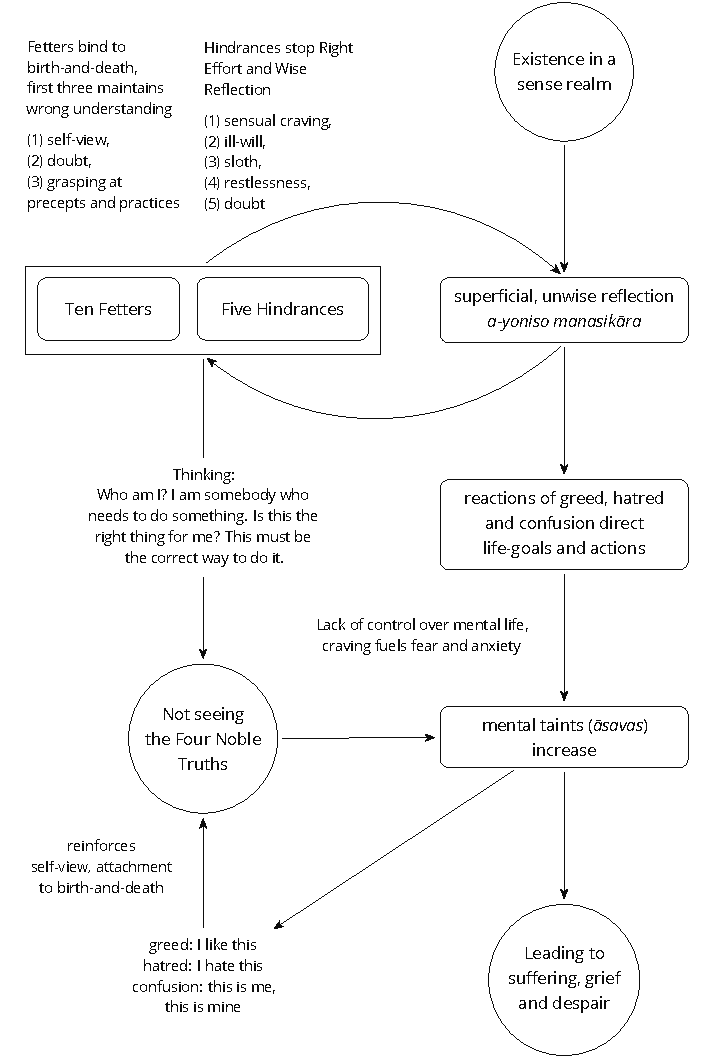
\includegraphics[width=80mm]{leading-to-suffering.pdf}

\end{figure}

\clearpage

\begin{figure}[h]
\caption{Leading to Cessation}\label{fig-leading-to-cessation}

\centering

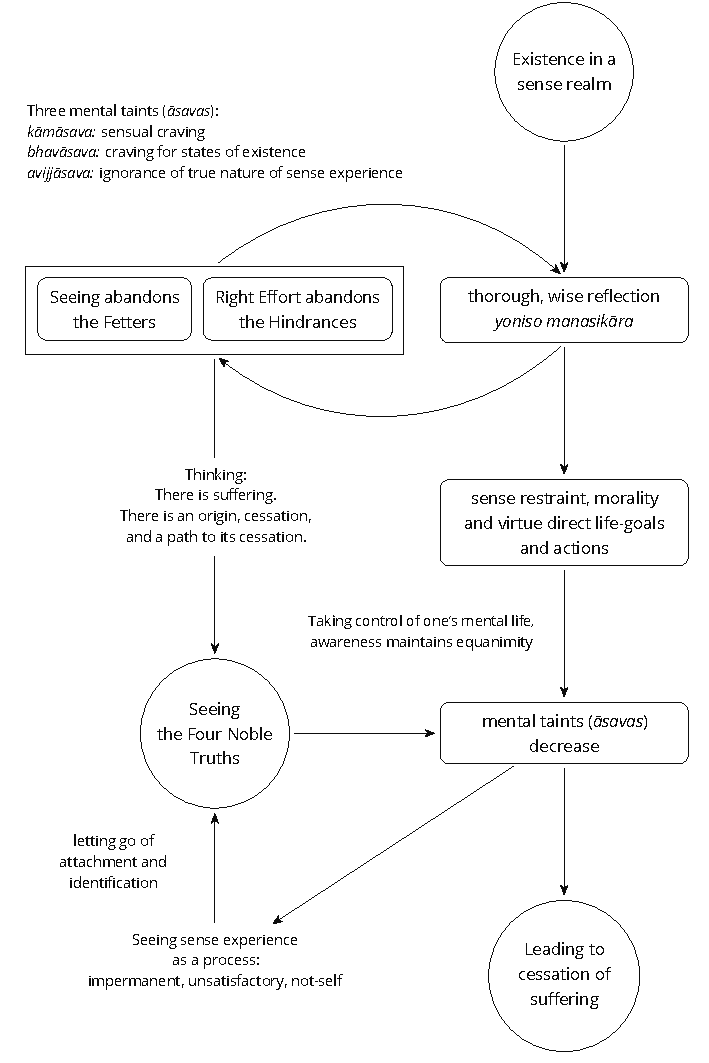
\includegraphics[width=80mm]{leading-to-cessation.pdf}

\end{figure}

\clearpage

\section{Right View}

\keywords{returning to the beginning, observing thoughts}

Let's return to the breathing and continuing the meditation practice.
Start the beginning of the session with the basics, simple steps which
guide the attention back to the familiar frame: the in- and out breath,
the body and its feelings. Observe what you are experiencing as a
process, which is going through continuos change from one feeling into
another. Every meditation session is a new beginning, we can't save the
results of the previous session and load in the knowledge. If we start
thinking we already know, say, if we have been practising this for
years, this results in a closed attitude which blocks even our earlier
understanding, because it is only relevant when applied to the present.
The changing present keeps understanding fresh and new.

This thought, this feeling had a beginning, it is changing now, it will
cease and end. Can I wait and notice that cessation?' Contemplating
direct experience this way, the mind gives up its desire and fear
regarding particular states, and understands them as part of natural
processes. We are not reasoning to ourselves what we think about the
mind, rather, as if taking a step back and watching it, we are mindfully
experiencing the way it is.

\enlargethispage*{\baselineskip}

This contemplation restores right view, as if someone took an upside
down flower vase, standing on its top, and put it upright again, and so
when we look we understand, which part of the vase is the top and the
bottom. We crave and want to hold onto experiences that are always going
to change; doesn't that sound like stress and suffering? Fortunately the
mistake is avoidable.

\clearpage

\keywords{freedom around limitations, essentials, gratitude, flooded with good advice}

Right view finds the space and freedom around the limitations and
pressures of life. At first we might not see much open space, but
contemplating the essentials we might notice that we may not need
everything we can think of. We can ask, `Do I have what we need to live
this single day?' Let's take stock of what we are using in our immediate
environment -- clothing, food, shelter, medicine. One time someone gives
it to us or allows us to use them, at other times we give them to
others. `Do I know what is enough to do today?' Although I might know
these fact already, I feel that a calmness returns when I recollect them
again.

With this simple fact that we have what we need to live this day well,
our attitude expresses itself in feeling contentment and gratitude for
life. You don't have to ask for it and you can't create it by will. We
have to make space for it in our view, then it arises on its own.

What is the great hurry for? A simple exercise is to stop for two
minutes, not looking for entertainment and distraction, doing nothing
for two minutes. You can watch to breath, but it's optional. Allowing
boredom as a mental state increases our focus and preserves energy.

The problem is not that we don't know enough. The bookshelves are
overflowing with good advice about `how to be happy', if that's all we
need, where is the problem? If all it took was good advice, all of us
would have been already enlightened long ago. We hear and read about all
the good things we should do, what sort of person we should be: one book
says we should be tough and fearless, while another says we should have
universal compassion. It is a special kind of suffering to read it all.

Or perhaps we need \emph{Nibbāna}? Is that the right thing? The meaning
of the word is \emph{going cool}, we may think of a fire ceasing to burn
and growing cool. A craving to `have it' would be more fuel for the heat
and burning of becoming. But \emph{Nibbāna} is the coolness of ceasing
to burn with becoming, so should we become this non-becoming? The
thinking mind goes, `\emph{What?!}' And that's not a wrong answer
either: the teaching of the Buddha points out that thinking and becoming
is not sufficient here. Another state or thought, when we see see
ourselves in it, will be as limiting as before. We are not free by
becoming the right thing, but by recognizing that we can give up the
compulsion to continue becoming.

\section{New Eyes}

\keywords{turning toward experience, intellectual knowledge, watching the senses}

We can turn a compulsive tendency into meditation practice by asking,
`How can I understand this experience?' This question directs us to the
noble attitude to suffering described in the Four Noble Truths:
`Suffering should be understood.' Discard the opinions which present
themselves as answers, and keep returning to this open attitude of
knowing the present.

Both joy and sorrow are natural processes, but if we don't understand
them, we see one as a reward and the other as punishment. Life never
seems to be fair and it always seems to be out of our control.

To open up our attitude for contemplation, we can at least imagine the
possibility that there is something here we can learn. A turning point
occurs when we are not sure about our opinions and when we stop to
investigate the experience itself. Consider how narrow our attitude is
when we start with the thought, `\emph{I've seen this, I know this}'.
Perhaps this is true, and I have seen and recognized it before. But I
notice that when I try to use that intellectual knowledge to solve a
problem, my attention revolves around memories, thoughts and opinions.
While I am caught up in the past, the present experience escapes my
attention.

The instruction of the Buddha is to establish a careful intention to
meditate, and to put aside the matters of the world. We are to watch
experiences directly as they are, in the body, feelings, mind, and their
natural processes.

\begin{quote}
There is the case where a monk remains focused \ldots{} ardent, alert,
and mindful -- subduing greed and distress with reference to the world.

\bigskip

\quoteRef{%

\href{https://suttacentral.net/mn10}{MN 10}, Mindfulness Meditation

}
\end{quote}

Contemplating our experience through watching the senses, noticing
impermanence changes our attitudes and perspectives. This is about
understanding a process, not about gaining knowledge. There is still no
fixed thought or opinion which will become `our knowledge'. Instead, our
trust is now in the awareness which can be conscious of, and stay with
the changing present. `\emph{What} is it that I am doing? \emph{How} am
I doing it?' Letting go of our fixed positions becomes the way forward;
we discover it by seeing with new eyes.\footnote{`The real voyage of
  discovery consists not in seeking new landscapes, but in having new
  eyes.' (Marcel Proust)} Life may still not be fair or entirely under
our control, but now we are familiar with a practice which makes the
difference between having a mental breakdown and facing the facts with
understanding.

It feels hopeless sometimes, and the thinking mind seems to have no way
to stop itself. The fundamental principle is that watching the mind
develops the mind. A wakeful, conscious awareness stops the compulsive
tendencies which have been unknown, unseen, and driving us into the same
old painful situations.

We don't know what is going to happen tomorrow, but there will be
change. The ideas which accord with this change will lead to happiness,
the ideas which are compulsive and rigid will lead to suffering. The
practice is not to accumulate or to gain knowledge, but learning to
trust our capacity to practise this wakeful awareness in the present,
which understands that change is an essential part of being alive.
Turning away from that change creates the fears and obstructions which
make us feel dead and meaningless. The word `Buddha' means `one who
knows, one who is awake'. The source of contentment in activity is that
we continue to trust and practice this wakeful awareness.
